\documentclass[dvipdfmx,autodetect-engine,titlepage]{jsarticle}
\usepackage[dvipdfm]{graphicx}
\usepackage{ascmac}
\usepackage{fancybox}
\usepackage{listings}
\usepackage{plistings}
\usepackage{itembkbx}
\usepackage{amsmath}
\usepackage{svg}
\usepackage{url}
\usepackage{graphics}
\usepackage{listings,jvlisting}
\usepackage{scalefnt}

\textheight=23cm
\renewcommand{\figurename}{図}
\renewcommand{\tablename}{表}
\newenvironment{code}
{\vspace{0.5zw}\VerbatimEnvironment  
\begin{screen} 
\baselineskip=1.0\normalbaselineskip
 \begin{Verbatim}}
{\end{Verbatim}
\baselineskip=\normalbaselineskip
 \end{screen}\vspace{0.5zw}} 

\title{情報理工学部 SNコース 2回\\
セキュリティ・ネットワーク学実験2\\
NW実験2-4レポート}
\author{2600200443-6\\Yamashita Kyohei\\山下 恭平}
\date{November 23 2021}

\begin{document}

\maketitle

\section{概要}
自宅のネットワーク環境,および学内ネットワーク環境において,指定された場所へ
のネットワーク経路を調べる。

\section{結果と考察}

\subsection{自宅のネットワーク}

\begin{figure}[htbp]
  \begin{tabular}{cc}
    \begin{minipage}[t]{0.45\hsize}
      \centering
      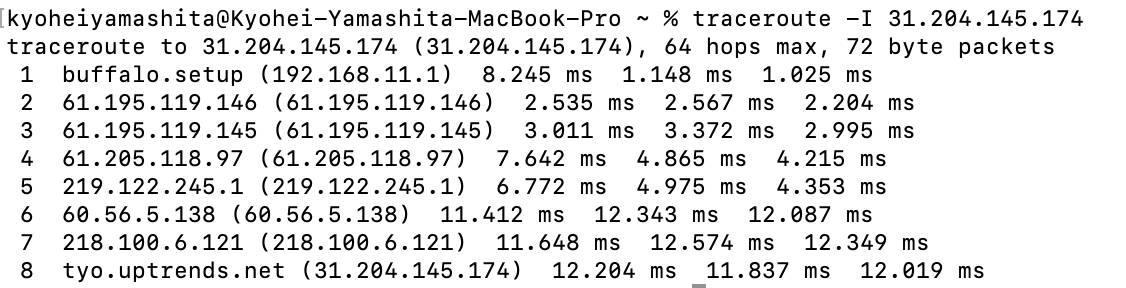
\includegraphics[keepaspectratio, scale=0.35]{SS5.png}
      \caption{東京}
    \end{minipage} &
    \begin{minipage}[t]{0.45\hsize}
      \centering
      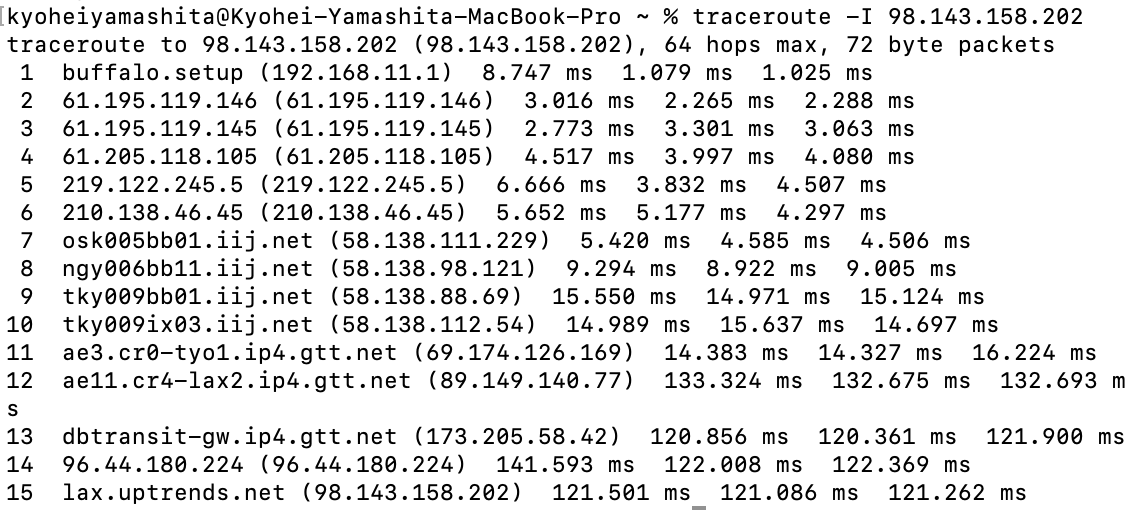
\includegraphics[keepaspectratio, scale=0.35]{SS6.png}
      \caption{アメリカ西海岸}
    \end{minipage} \\ \\ \\
 
    \begin{minipage}[t]{0.45\hsize}
      \centering
      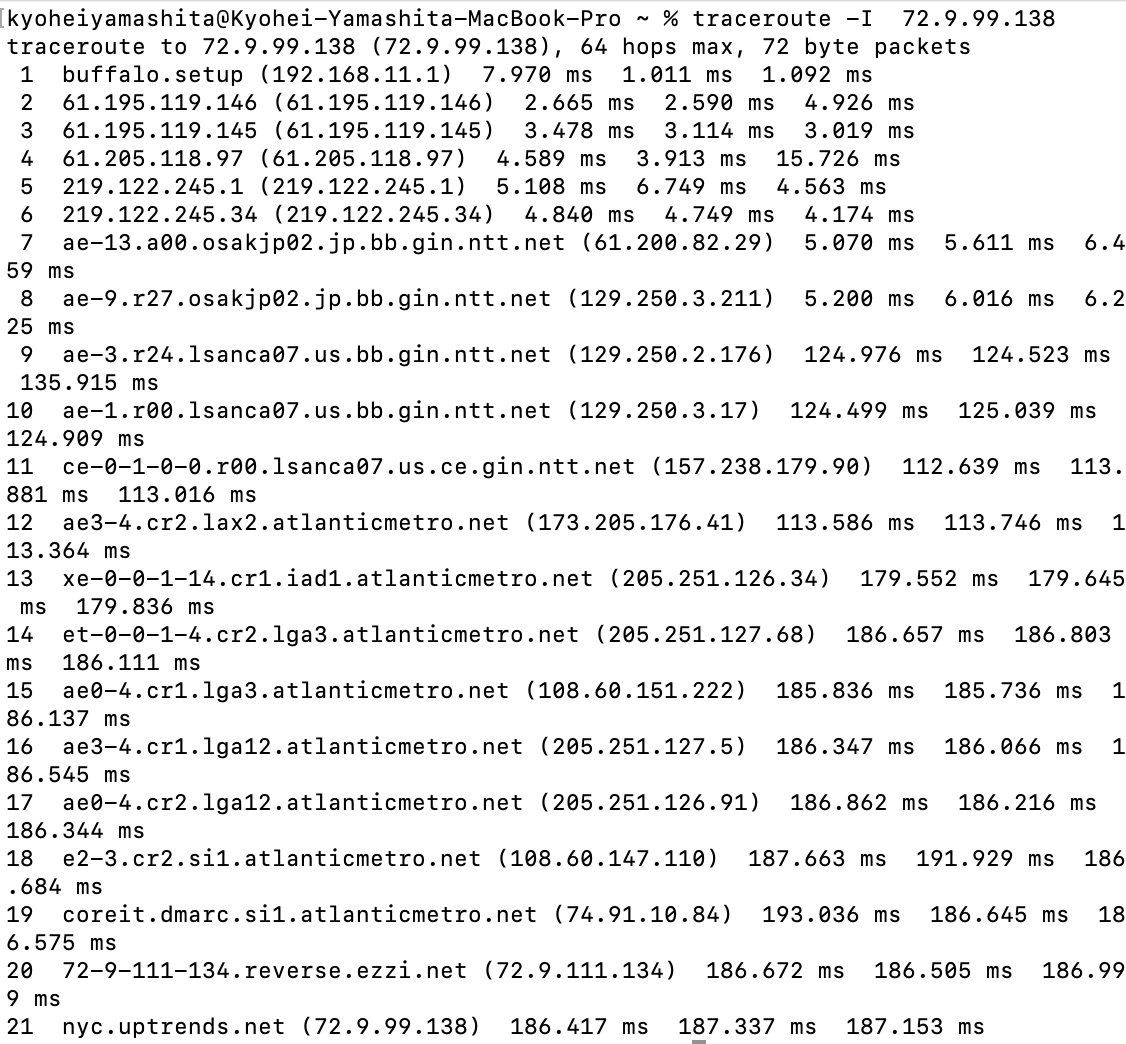
\includegraphics[keepaspectratio, scale=0.35]{SS7.png}
      \caption{アメリカ東海岸}
    \end{minipage} &
    \begin{minipage}[t]{0.45\hsize}
      \centering
      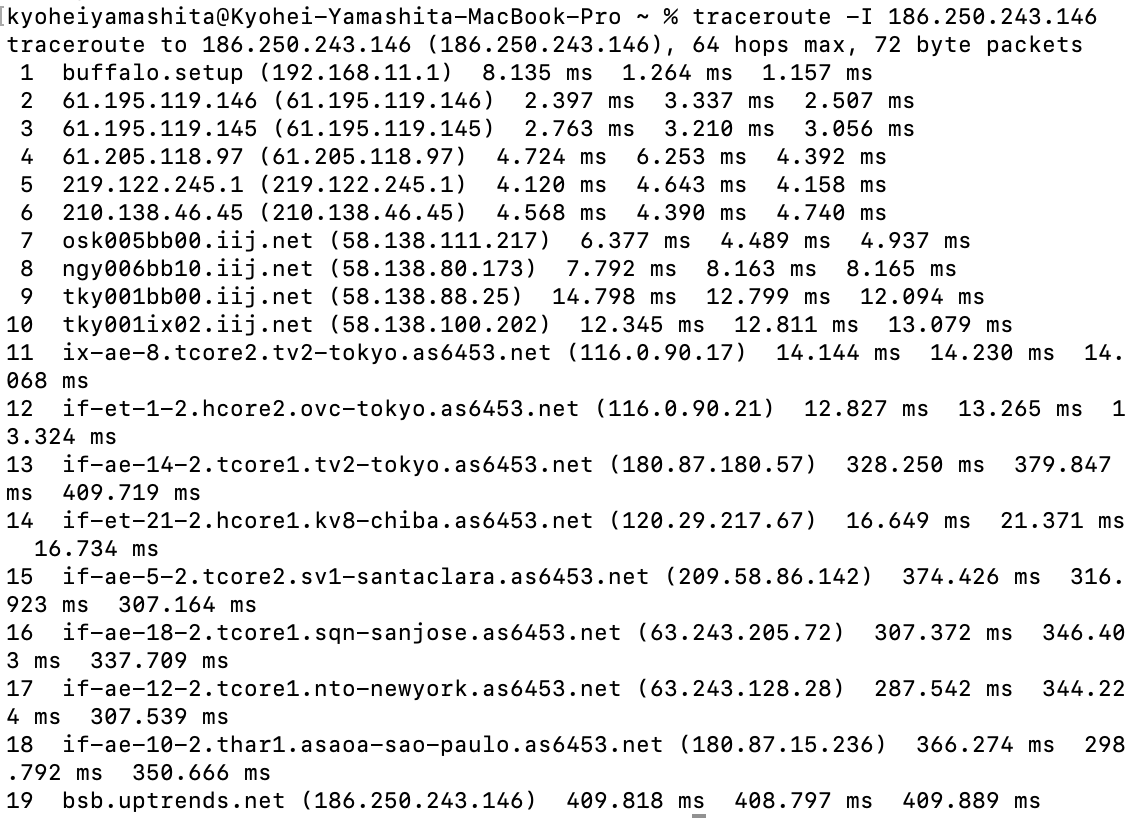
\includegraphics[keepaspectratio, scale=0.35]{SS8.png}
      \caption{ブラジル}
    \end{minipage}
  \end{tabular}
\end{figure}

入力した結果は上の図に示した。\\
全ての結果に共通している部分は初めの3行であり、1行目は自宅のWi-Fiルータであ
る。2,3行目は調べたところプロバイダの会社によるルータであったので、自宅
近くに存在するルータだと考えられる。また、5行目までのIPアドレスはどれも
似ていることから、これらも契約プロバイドのルータであり、6行目以降から目的
のサーバ、ルータに向かっていると考えられる。\\
アメリカ西海岸では11行目でアメリカのサーバにアクセスしていおり、そこから4つの
中継で目的のサーバに到達しているが、東海岸では8行目でアメリカのサーバに
アクセスしているのにもかかわらず到達まで13個の中継をしている、これは8行目
ではまだ西海岸であり、そこから東海岸までアメリカ国内のサーバを中継しているから
と考えられる。ブラジルでは日本からアメリカ西海岸、東海岸を経てブラジルのサーバへ
アクセスしていることが実行結果から読み取れる。実際には、日本、サンタクララ、サンノゼ
、ニューヨーク、サンパウロそして、目的のサーバへと到達していることがわかる。



\subsection{学内ネットワーク}
全ての結果を以下に示した。\\
全てに共通している一行目の「172.31.191.253」はBKC内にあるルータだと
考えられる。情報理工学部実験用サーバおよびBKCのDNSサーバは、同じくBKC内
に存在し、同一LAN上にあると考えられるの、2行目の時点で目的のサーバに到着
していることがわかる。\\
衣笠および立命館慶祥のDNSサーバは2回では到着していないことから、少なくとも
BKC内には存在しないと考えられる。しかし、中継しているIPアドレスがかなり
似ていることから、キャンパス同士のネットワークも接続されていることが考え
られる。

\begin{figure}[htbp]
  \begin{tabular}{cc}
    \begin{minipage}[t]{0.45\hsize}
      \centering
      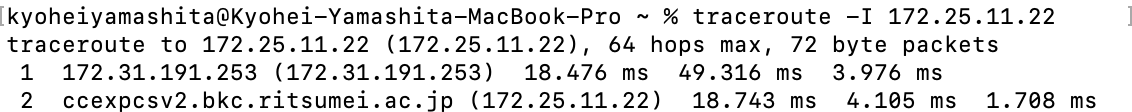
\includegraphics[keepaspectratio, scale=0.35]{SS1.png}
      \caption{情報理工学部実験用サーバ}
    \end{minipage} &
    \begin{minipage}[t]{0.45\hsize}
      \centering
      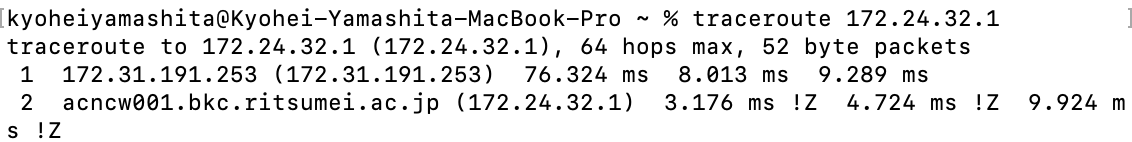
\includegraphics[keepaspectratio, scale=0.35]{SS2.png}
      \caption{BKCのDNSサーバ}
    \end{minipage} \\ \\ \\
 
    \begin{minipage}[t]{0.45\hsize}
      \centering
      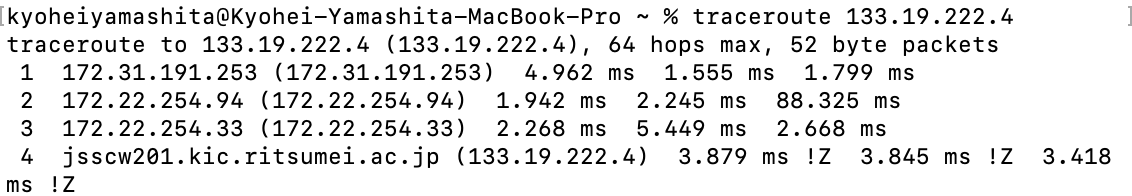
\includegraphics[keepaspectratio, scale=0.35]{SS3.png}
      \caption{衣笠のDNSサーバ}
    \end{minipage} &
    \begin{minipage}[t]{0.45\hsize}
      \centering
      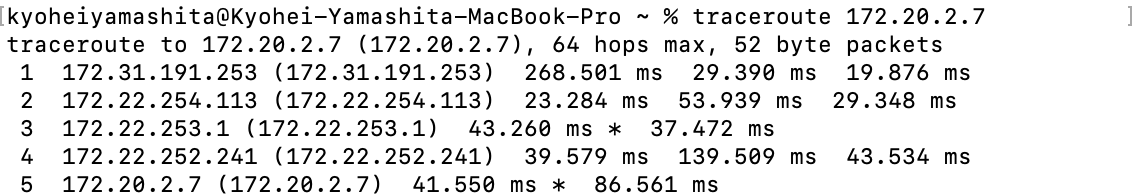
\includegraphics[keepaspectratio, scale=0.35]{SS4.png}
      \caption{立命館慶祥高校のDNSサーバ}
    \end{minipage}
  \end{tabular}
\end{figure}

\section{地理的距離とネットワークの関係性について}
地理的にホストが近くても、ネットワーク的には近いとは限らない理由として考え
られるのは、目的のホストへ到達するためのルータやサーバが地理的に近くにあると
は限らないからである。例えば、大津市のホームページまでの経路を考えたとき、
最終的にはもちろん大津市にあるサーバに到着するが、私の場合、プロバイダのサーバ
が大阪にあるので、必ず大阪を経由する。このように、地理的に近いホストであっても
ネットワーク的には近くないことが起こると考えられる。

\end{document}

